\documentclass[border=6pt]{standalone}
\usepackage{amsmath}
\usepackage{tikz}
\usetikzlibrary{arrows.meta}
\begin{document}
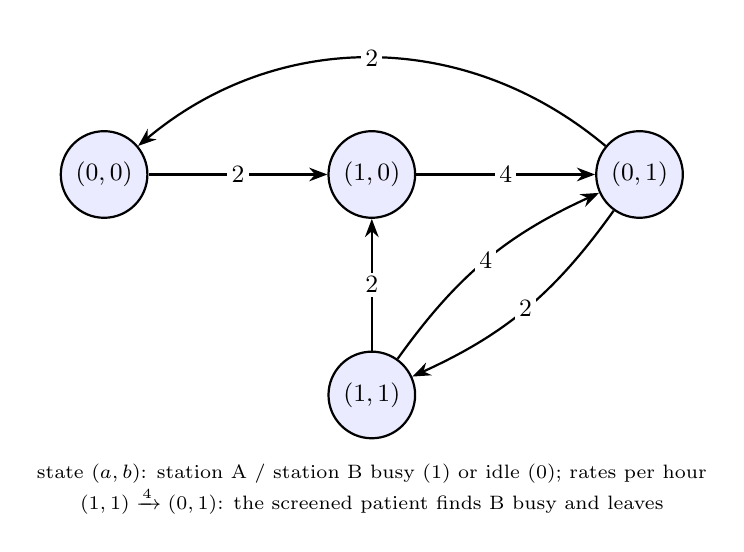
\begin{tikzpicture}[>=Stealth,font=\small,
 s/.style={draw,thick,circle,minimum size=1.1cm,inner sep=0pt,fill=blue!8},
 e/.style={->,thick},
 lab/.style={font=\small,fill=white,inner sep=1.5pt},
 every loop/.style={->,thick,looseness=6}]
\node[s] (00) at (0,0) {$(0,0)$};
\node[s] (10) at (3.4,0) {$(1,0)$};
\node[s] (01) at (6.8,0) {$(0,1)$};
\node[s] (11) at (3.4,-2.8) {$(1,1)$};
\draw[e] (00) -- node[lab]{2} (10);
\draw[e] (10) -- node[lab]{4} (01);
\draw[e] (01) to[bend right=40] node[lab]{2} (00);
\draw[e] (01) to[bend left=15] node[lab]{2} (11);
\draw[e] (11) to[bend left=15] node[lab]{4} (01);
\draw[e] (11) -- node[lab]{2} (10);
\node[font=\scriptsize,align=center] at (3.4,-4.0) {state $(a,b)$: station A / station B busy (1) or idle (0); rates per hour\\$(1,1)\xrightarrow{4}(0,1)$: the screened patient finds B busy and leaves};
\end{tikzpicture}
\end{document}
